\section{Closed Innovation}\label{sec:grundlagen-closed}

\subsection{Ursprung}
Das \textit{Closed Innovation}-Modell ist das vorherrschende Innovationsmodell im 20. Jahrhundert.
Es spiegelt die damalige Wissensumgebung wider.
Unter Wissenschaftlern ist es verpönt ihre Fähigkeiten zu nutzen, um wirtschaftliche Probleme zu lösen.

Um dennoch Innovationen anzutreiben und so den kommerziellen Erfolg zu sichern,
sind Unternehmen gezwungen selbst in \ac{fe} zu investieren.
Da auch bei Zulieferern das notwendige Wissen nicht aufgebaut ist,
müssen Unternehmen innerhalb ihrer \ac{fe}-Organisation das gesamte Spektrum von den Grundlagen bis hin zum fertigen Produkt abdecken.
Voraussetzung hierfür ist die Akquise von talentierten Mitarbeitern.

\subsection{Prinzipien}
Implizit ergeben sich so die Prinzipien der \textit{Closed Innovation} (nach \cite[19]{herzog2011}):
\begin{itemize}
    \item Ein Unternehmen sollte die talentiertesten Mitarbeiter anstellen.
    \item Um von Innovationen zu profitieren, müssen diese innerhalb des Unternehmens den gesamten Innovationsprozess durchlaufen. (Vom Entdecken, über das Entwickeln bis hin zur Vermarktung)
    \item Um ein Produkt als erstes auf den Markt zu bringen, muss eine Entdeckung innerhalb des eigenen Unternehmens entstehen.
    \item Bringt ein Unternehmen ein Produkt zuerst auf den Markt, so gewinnt es den Wettbewerb.
    \item Investiert ein Unternehmen am meisten in \ac{fe}, so entstehen dort die besten Ideen, was wiederum den Wettbewerb gewinnt.
    \item Damit andere Unternehmen nicht von den eigenen Entdeckungen profitieren, gilt es das geistige Eigentum zu schützen.
\end{itemize}

\subsection{Modell}
Aus diesen Regeln folgt das in \autoref{fig:closedInnovation} dargestellte Modell.
Der gesamte Innovationsprozess spielt sich innerhalb der Grenzen des Unternehmens ab.
Eine Innovation beginnt immer mit einer Idee innerhalb des Unternehmens,
wird durch die firmeneigene \ac{fe}-Abteilung entwickelt
und schließlich auf dem bestehenden Markt des Unternehmens kommerzialisiert.

\begin{figure}[ht!]
    \centering
    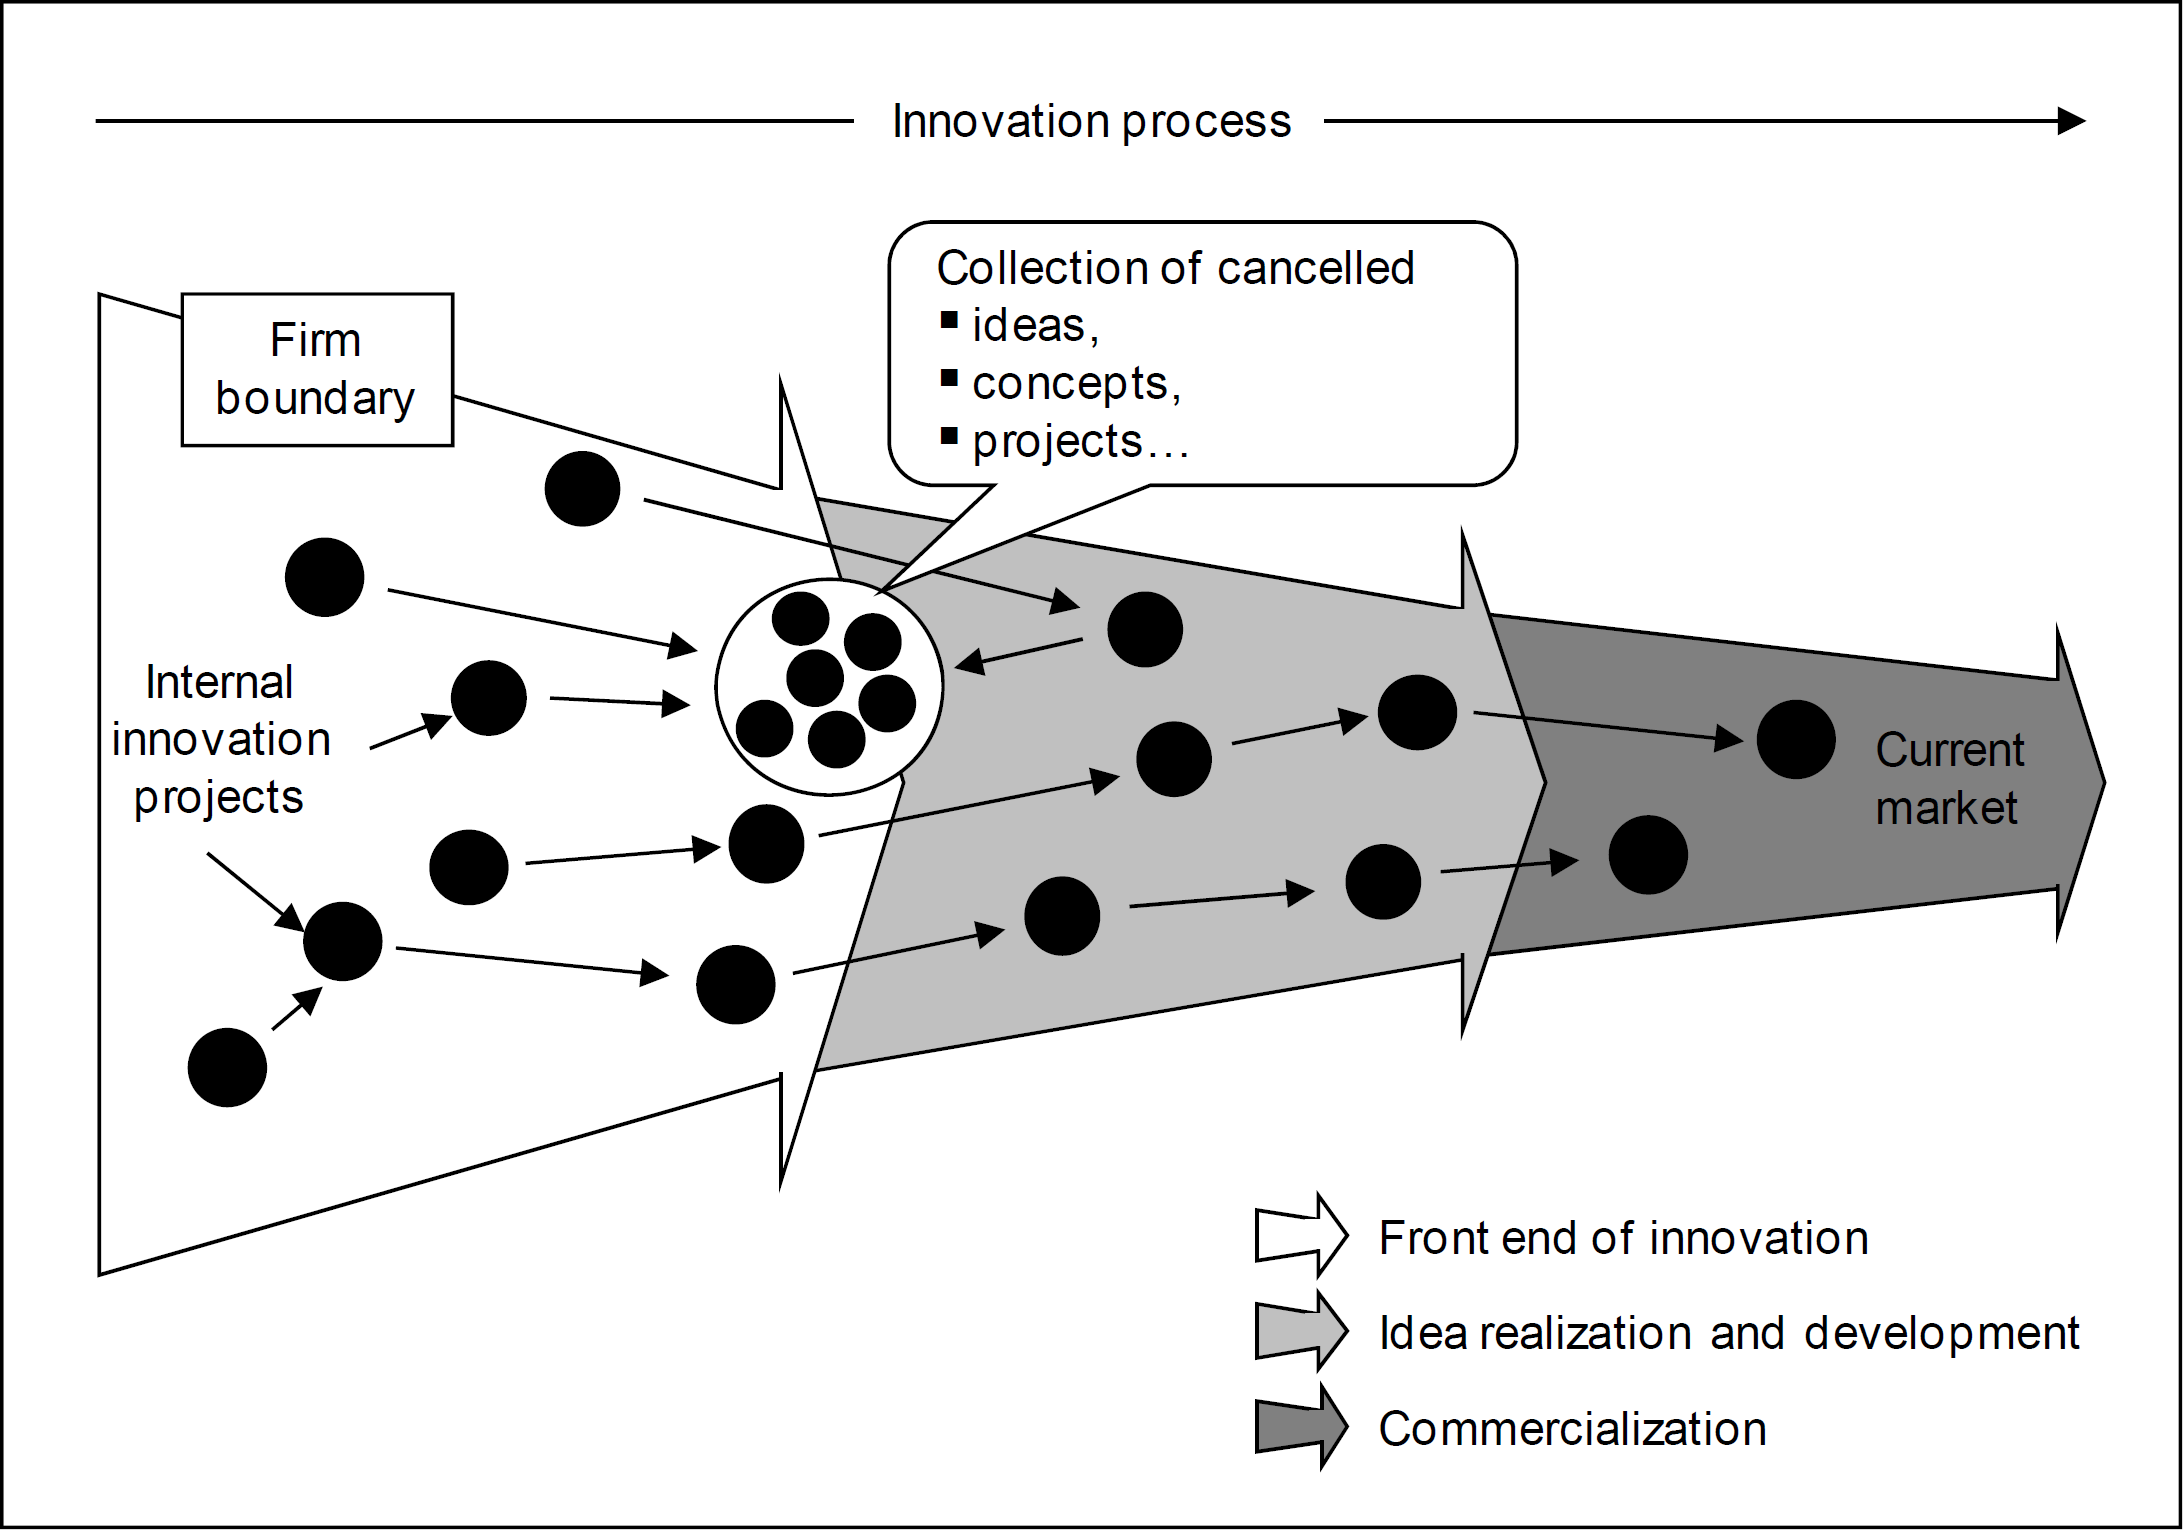
\includegraphics[width=1\textwidth]{ClosedInnovation}
    \caption{Closed Innovation Modell (aus \cite[20]{herzog2011})}
    \label{fig:closedInnovation}
\end{figure}

Nicht alle Ideen können realisiert werden.
Einerseits ist dies ist darauf zurückzuführen, dass Ressourcen in Form von Arbeitskraft oder Wissen nicht ausreichend vorhanden sind.
Andererseits zielt die Idee nicht auf den aktuellen Markt oder es wird vermutet, dass dort keine Akzeptanz herrscht.

Abgelehnte Ideen und abgebrochene Projekte werden beispielsweise in Datenbanken gesammelt.
Von dort werden sie wieder aufgegriffen
oder bleiben ein ungenutzter Teil des geistigen Eigentums eines Unternehmens.


